% automatically generated document using lt2circuiTikz
\documentclass[tikz,margin={2pt 2pt 2pt 2pt}]{standalone}
\usepackage[compatibility,siunitx,  americanvoltages, americancurrents, europeanresistors, europeaninductors, americanports,%
  straightlabels, fetbodydiode, straightvoltages]{circuitikz}
\usepackage{tikz,amsmath, amssymb,bm,color,pgfkeys,siunitx,ifthen,ulem}
\usepackage{pgfplots}
\pgfplotsset{compat=1.14}
\usetikzlibrary{shapes,arrows}
%\usepackage{agaramondc}					% Adobe Garamond, custom shape
%\renewcommand{\shapedefault}{rtl} % rtl: roman tabular lining

\makeatletter

%% bandstop filter (adapted from highpass)
\pgfcircdeclarebipole{}{\ctikzvalof{bipoles/highpass/width}}{*bandstop}{\ctikzvalof{bipoles/highpass/width}}{\ctikzvalof{bipoles/highpass/width}}{
	\pgf@circ@res@step = \ctikzvalof{bipoles/highpass/width}\pgf@circ@Rlen
	\divide \pgf@circ@res@step by 2
	
	\pgfpathmoveto{\pgfpoint{\pgf@circ@res@left}{\pgf@circ@res@zero}}
	\pgf@circ@res@other = \pgf@circ@res@left
	\advance\pgf@circ@res@other by \pgf@circ@res@step 
	
	\ifpgf@circuit@dashed
	\pgfsetdash{{0.1cm}{0.1cm}}{0cm} 
	\fi	
	
	% draw outer box
	\pgfsetlinewidth{\pgfkeysvalueof{/tikz/circuitikz/bipoles/thickness}\pgfstartlinewidth}
	\pgfpathrectanglecorners{\pgfpoint{\pgf@circ@res@left}{\pgf@circ@res@up}}{\pgfpoint{\pgf@circ@res@right}{\pgf@circ@res@down}}
	\pgfusepath{draw}
	
	\ifpgf@circuit@inputarrow
	{
		\advance \pgf@circ@res@left by -.5\pgfkeysvalueof{/tikz/circuitikz/bipoles/thickness}\pgfstartlinewidth
		\pgftransformshift{\pgfpoint{\pgf@circ@res@left}{0pt}}
		\pgfnode{inputarrow}{tip}{}{pgf@inputarrow}{\pgfusepath{fill}}
	}
	\fi
	
	% rotate inner symbol
	\def\pgfcircmathresult{\expandafter\pgf@circ@stripdecimals\pgf@circ@direction\pgf@nil}
	\ifnum \pgfcircmathresult > 45 \ifnum \pgfcircmathresult < 135
	\pgftransformrotate{270}
	\fi\fi
	\ifnum \pgfcircmathresult > 134 \ifnum \pgfcircmathresult < 225  % 134 degree, because >= 135 is not possible
	\pgftransformrotate{180}
	\fi\fi
	\ifnum \pgfcircmathresult > 224 \ifnum \pgfcircmathresult < 315
	\pgftransformrotate{90}
	\fi\fi
	
	% draw inner symbol
	\pgfsetdash{}{0pt}	% always draw solid line for inner symbol
	\pgfsetarrows{-} %never draw arrows
	\pgfsetlinewidth{\pgfstartlinewidth}
	\pgfpathmoveto{\pgfpoint{-0.5\pgf@circ@res@step}{0.5\pgf@circ@res@step}}
	\pgfpathsine{\pgfpoint{.25\pgf@circ@res@step}{.25\pgf@circ@res@step}}
	\pgfpathcosine{\pgfpoint{.25\pgf@circ@res@step}{-.25\pgf@circ@res@step}}
	\pgfpathsine{\pgfpoint{.25\pgf@circ@res@step}{-.25\pgf@circ@res@step}}
	\pgfpathcosine{\pgfpoint{.25\pgf@circ@res@step}{.25\pgf@circ@res@step}}
	\pgfusepath{draw}
	
	\pgfpathmoveto{\pgfpoint{-0.5\pgf@circ@res@step}{0}}
	\pgfpathsine{\pgfpoint{.25\pgf@circ@res@step}{.25\pgf@circ@res@step}}
	\pgfpathcosine{\pgfpoint{.25\pgf@circ@res@step}{-.25\pgf@circ@res@step}}
	\pgfpathsine{\pgfpoint{.25\pgf@circ@res@step}{-.25\pgf@circ@res@step}}
	\pgfpathcosine{\pgfpoint{.25\pgf@circ@res@step}{.25\pgf@circ@res@step}}
	\pgfusepath{draw}
	\pgfpathmoveto{\pgfpoint{-0.15\pgf@circ@res@step}{-0.15\pgf@circ@res@step}}
	\pgfpathlineto{\pgfpoint{0.15\pgf@circ@res@step}{0.15\pgf@circ@res@step}}
	\pgfusepath{draw}
	
	\pgfpathmoveto{\pgfpoint{-0.5\pgf@circ@res@step}{-0.5\pgf@circ@res@step}}
	\pgfpathsine{\pgfpoint{.25\pgf@circ@res@step}{.25\pgf@circ@res@step}}
	\pgfpathcosine{\pgfpoint{.25\pgf@circ@res@step}{-.25\pgf@circ@res@step}}
	\pgfpathsine{\pgfpoint{.25\pgf@circ@res@step}{-.25\pgf@circ@res@step}}
	\pgfpathcosine{\pgfpoint{.25\pgf@circ@res@step}{.25\pgf@circ@res@step}}
	\pgfusepath{draw}
	%	\pgfpathmoveto{\pgfpoint{-0.15\pgf@circ@res@step}{-0.65\pgf@circ@res@step}}
	%	\pgfpathlineto{\pgfpoint{0.15\pgf@circ@res@step}{-0.35\pgf@circ@res@step}}
	%	\pgfusepath{draw}
}

\tikzset{
	*bandstop/.style={\circuitikzbasekey, /tikz/to path=\pgf@circ@*bandstop@path},
}
\def\pgf@circ@*bandstop@path#1{\pgf@circ@bipole@path{*bandstop}{#1}}




\makeatother

\usetikzlibrary{backgrounds,calc,positioning}

\usetikzlibrary{circuits.ee.IEC}
\usetikzlibrary{arrows}


% sym32a style

\ctikzset{tripoles/mos style/arrows}
\ctikzset{
	/tikz/circuitikz/quadpoles/coupler/width=1,%1.3
	/tikz/circuitikz/quadpoles/coupler/height=0.952,%1.3
	/tikz/circuitikz/quadpoles/coupler2/width=1,%1.3
	/tikz/circuitikz/quadpoles/coupler2/height=0.952,%1.3
	/tikz/circuitikz/quadpoles/transformer/width=1.425,%1.5
	/tikz/circuitikz/quadpoles/transformer/height=1.425,%1.5
	/tikz/circuitikz/quadpoles/transformer core/width=1.425,%1.5
	/tikz/circuitikz/quadpoles/transformer core/height=1.425,%1.5
	/tikz/circuitikz/quadpoles/gyrator/width=1.425,%1.5
	/tikz/circuitikz/quadpoles/gyrator/height=1.425,%1.5
	%/tikz/circuitikz/monopoles/tlinestub/width=0.1875,%0.25 no effect!
	/tikz/circuitikz/tripoles/american and port/height=0.95,%.8
	/tikz/circuitikz/tripoles/american nand port/height=0.95,%.8
	/tikz/circuitikz/tripoles/american or port/height=0.95,%.8
	/tikz/circuitikz/tripoles/american nor port/height=0.95,%.8
	/tikz/circuitikz/tripoles/american xor port/height=0.95,%.8
	/tikz/circuitikz/tripoles/american xnor port/height=0.95,%.8
	/tikz/circuitikz/bipoles/tline/height=0.4,%0.3
%	/tikz/circuitikz/bipoles/tline/width=1.2,%0.8
	/tikz/circuitikz/bipoles/diode/height=0.375,%
	/tikz/circuitikz/bipoles/diode/width=0.375,%
	/tikz/circuitikz/bipoles/varcap/height=0.375,%
	/tikz/circuitikz/bipoles/varcap/width=0.375,%
	/tikz/circuitikz/tripoles/triac/height=1.05,%
	/tikz/circuitikz/tripoles/triac/width=0.952,%
	/tikz/circuitikz/tripoles/thyristor/height=1.05,%
	/tikz/circuitikz/tripoles/thyristor/width=0.952,%
	/tikz/circuitikz/tripoles/op amp/height=0.952,%
	/tikz/circuitikz/tripoles/op amp/width=1.2,%
	/tikz/circuitikz/tripoles/op amp/font=\footnotesize,
	/tikz/circuitikz/tripoles/gm amp/height=0.952,% 1.7
	/tikz/circuitikz/tripoles/gm amp/width=1.2,% 1.4
	%	/tikz/circuitikz/tripoles/gm amp/font=\footnotesize,
	/tikz/circuitikz/tripoles/plain amp/height=0.952,% 1.7
	/tikz/circuitikz/tripoles/plain amp/width=1.2,% 1.4
	/tikz/circuitikz/bipoles/resistor/voltage/straight label distance/.initial=.8,
	/tikz/circuitikz/bipoles/generic/voltage/straight label distance/.initial=.8,
	/tikz/circuitikz/bipoles/inductor/voltage/straight label distance/.initial=.8,
	/tikz/circuitikz/bipoles/fullgeneric/voltage/straight label distance/.initial=.8,
	/tikz/circuitikz/bipoles/capacitor/voltage/straight label distance/.initial=1.0,
	/tikz/circuitikz/bipoles/thickness=1.6,
}
\ctikzset{v/.append style={/tikz/european voltages}}

\definecolor{netlabelcolor}{rgb}{0, 0, 0.25}
\definecolor{lttotitextcolor}{rgb}{0, 0.4, 0.25}
\definecolor{lttotidrawcolor}{rgb}{0.6, 0.6, 0.6}
\definecolor{netcolor}{rgb}{0, 0, 0.5}

\pgfkeys{/lt2ti/netlabel/font/.initial= \small}
\pgfkeys{/lt2ti/text/font/.initial= \small}

\pgfkeys{/lt2ti/Net/.style= {netcolor}}
\tikzstyle{dashdotdotted}=[dash pattern=on 3pt off 2pt on \the\pgflinewidth off 2pt on \the\pgflinewidth off 2pt]

\pgfkeys{/lt2ti/VArrow/.style= {->,>=latex}}
\pgfkeys{/lt2ti/SArrow/.style= {->,>=angle 90}}

\begin{document}%
	%\centering%
		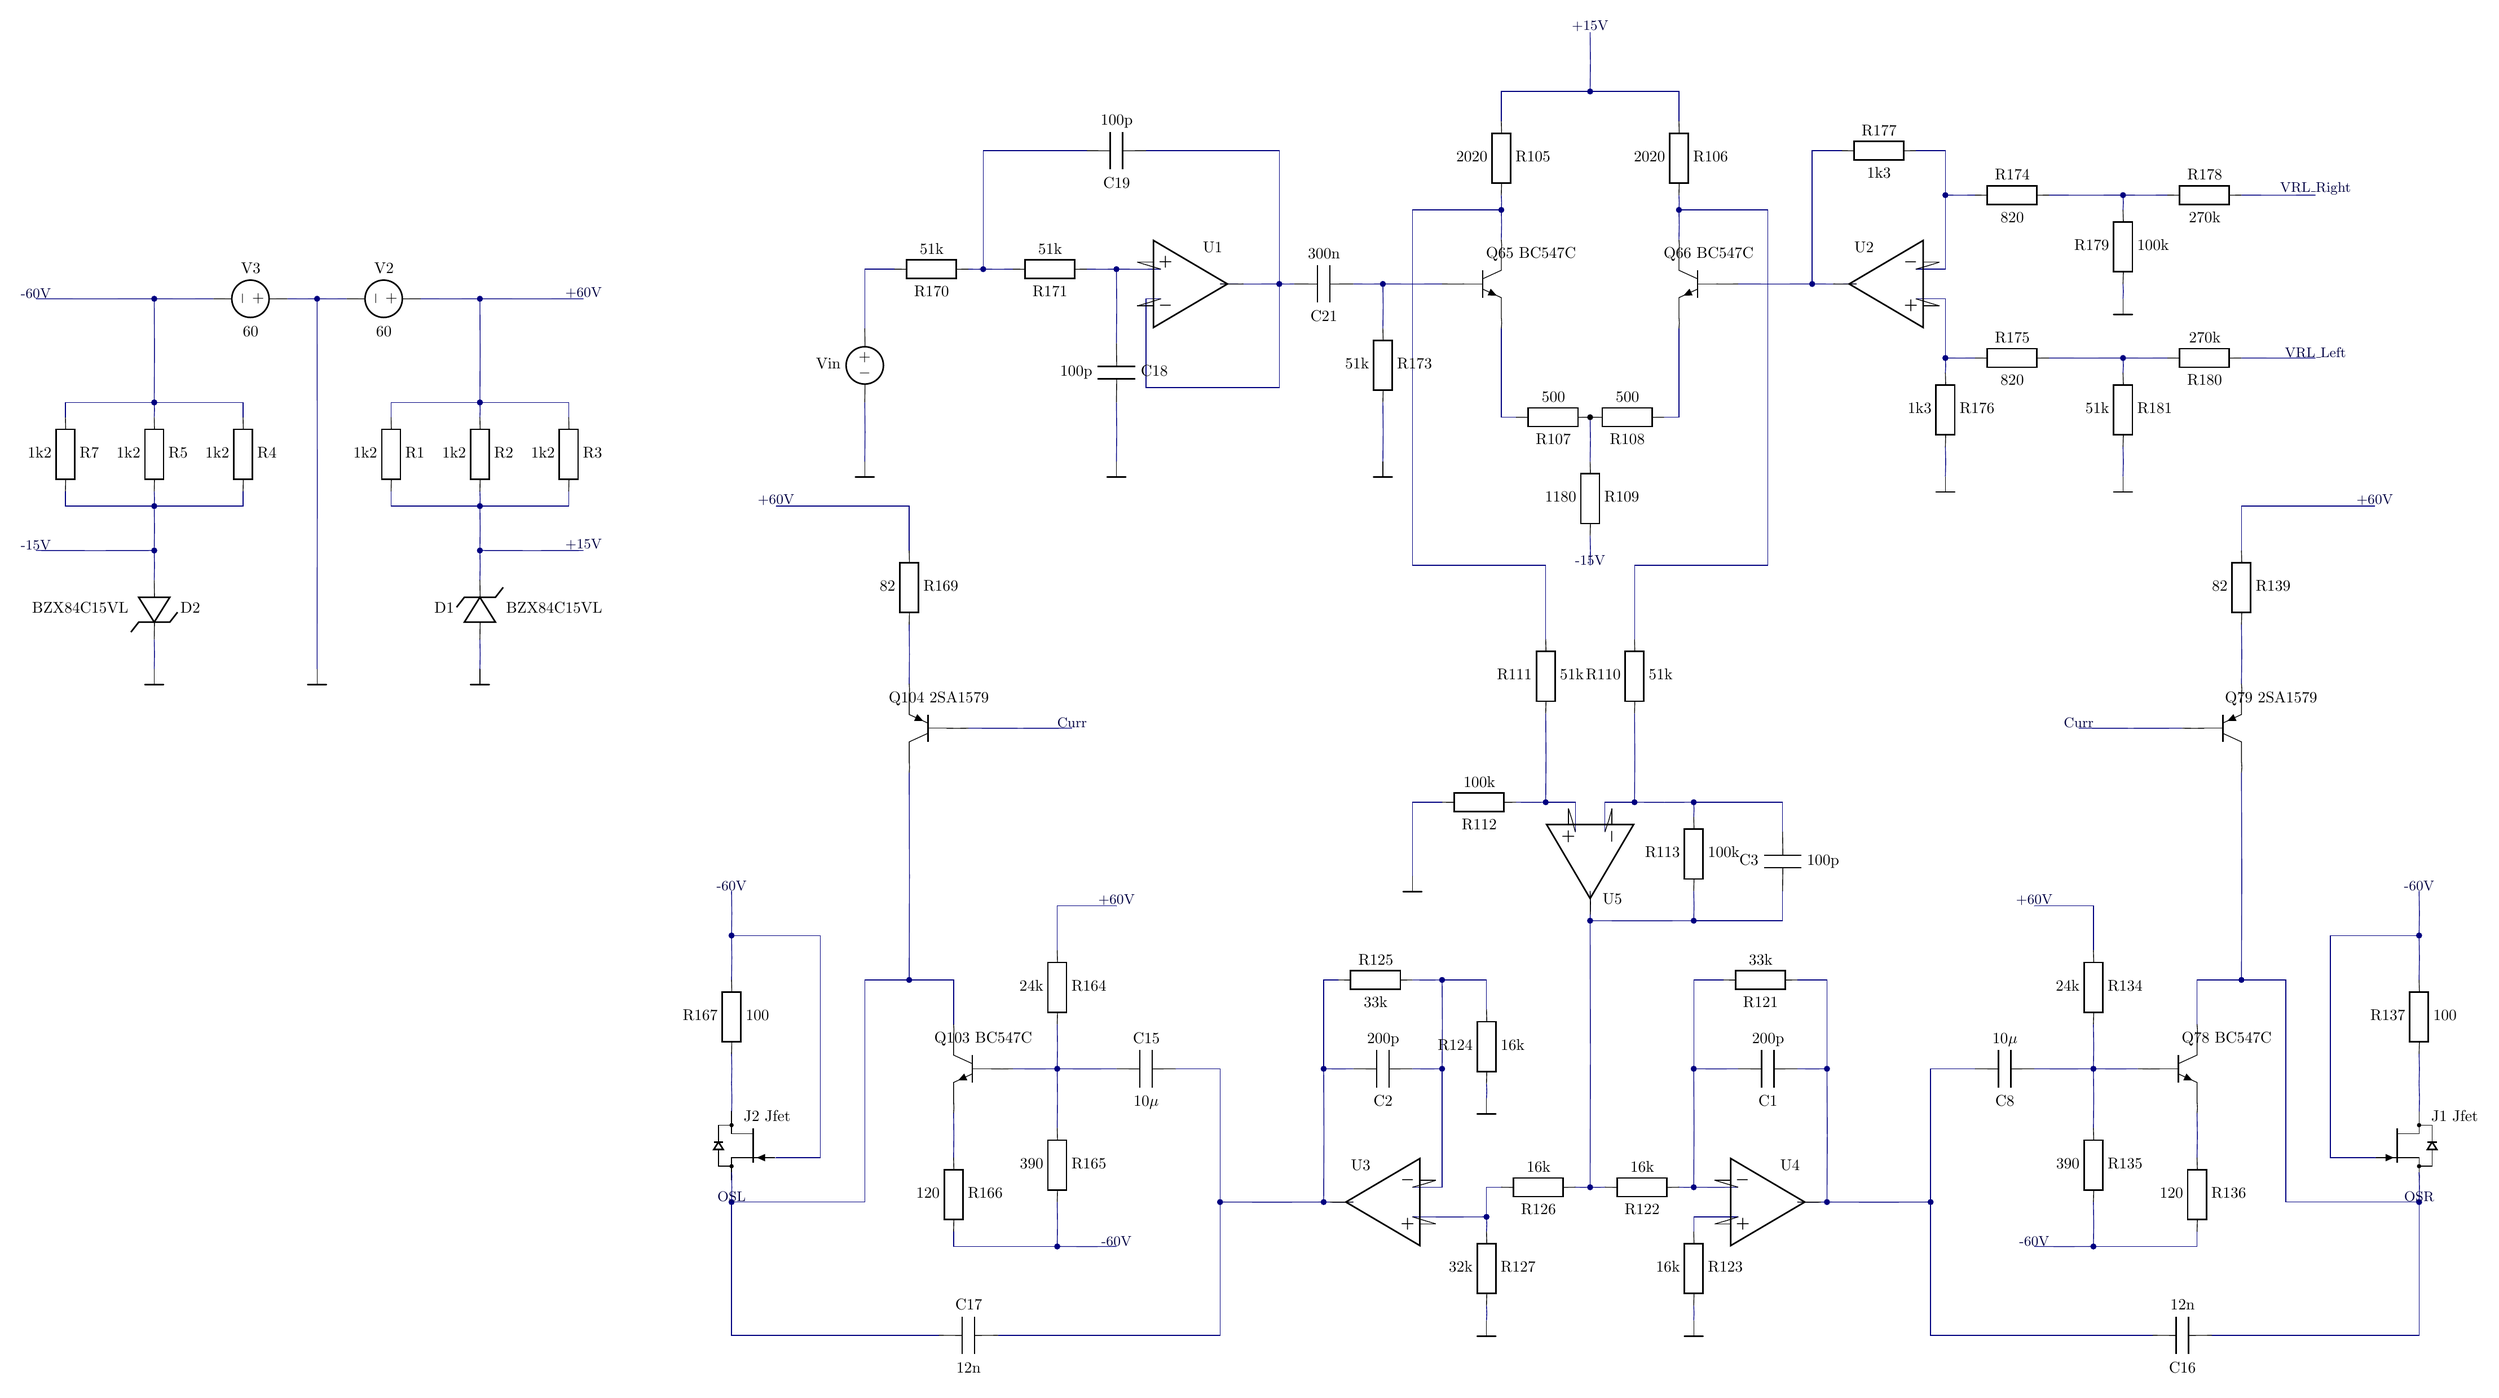
\begin{tikzpicture}[circuit ee IEC, scale=0.6666666667,line width=.5pt]% default: 0.4
	%\tikzstyle{every node}=[font=\small];%
	%\node [draw] at (0.0,0.0) {\pgfkeysvalueof{/tikz/circuitikz/tripoles/op amp/font}};
\draw [/lt2ti/Net](278.5,-83.0)to[*short,*-, color=netcolor] (278.5,-81.0);% wire w3
\draw [/lt2ti/Net](278.5,-83.0)to[*short,*-, color=netcolor] (278.5,-83.0);% wire w4_w6 start
\draw [/lt2ti/Net](275.5,-84.0)to[*short,-, color=netcolor] (275.5,-84.0);% wire w4_w6 end
\draw [/lt2ti/Net](278.5,-83.0) --  (275.5,-83.0) -- (275.5,-84.0); % wire w4_w6 polyline 
\draw [/lt2ti/Net](281.5,-84.0)to[*short,-, color=netcolor] (281.5,-84.0);% wire w5_w7 start
\draw [/lt2ti/Net](278.5,-83.0)to[*short,-*, color=netcolor] (278.5,-83.0);% wire w5_w7 end
\draw [/lt2ti/Net](281.5,-84.0) --  (281.5,-83.0) -- (278.5,-83.0); % wire w5_w7 polyline 
\draw [/lt2ti/Net](261.5,-85.0)to[*short,-, color=netcolor] (261.5,-85.0);% wire w8_w25 start
\draw [/lt2ti/Net](258.0,-89.0)to[*short,-*, color=netcolor] (258.0,-89.0);% wire w8_w25 end
\draw [/lt2ti/Net](261.5,-85.0) --  (258.0,-85.0) -- (258.0,-89.0); % wire w8_w25 polyline 
\draw [/lt2ti/Net](287.0,-85.0)to[*short,-, color=netcolor] (287.0,-85.0);% wire w10_w37 start
\draw [/lt2ti/Net](286.0,-89.5)to[*short,-*, color=netcolor] (286.0,-89.5);% wire w10_w37 end
\draw [/lt2ti/Net](287.0,-85.0) --  (286.0,-85.0) -- (286.0,-89.5); % wire w10_w37 polyline 
\draw [/lt2ti/Net](290.5,-86.5)to[*short,*-, color=netcolor] (290.5,-86.5);% wire w11_w12 start
\draw [/lt2ti/Net](289.5,-85.0)to[*short,-, color=netcolor] (289.5,-85.0);% wire w11_w12 end
\draw [/lt2ti/Net](290.5,-86.5) --  (290.5,-85.0) -- (289.5,-85.0); % wire w11_w12 polyline 
\draw [/lt2ti/Net](290.5,-86.5)to[*short,*-, color=netcolor] (290.5,-86.5);% wire w30_w31 start
\draw [/lt2ti/Net](289.5,-89.0)to[*short,-, color=netcolor] (289.5,-89.0);% wire w30_w31 end
\draw [/lt2ti/Net](290.5,-86.5) --  (290.5,-89.0) -- (289.5,-89.0); % wire w30_w31 polyline 
\draw [/lt2ti/Net](291.5,-86.5)to[*short,-*, color=netcolor] (290.5,-86.5);% wire w13
\draw [/lt2ti/Net](296.5,-86.5)to[*short,*-, color=netcolor] (294.0,-86.5);% wire w14
\draw [/lt2ti/Net](298.0,-86.5)to[*short,-*, color=netcolor] (296.5,-86.5);% wire w15
\draw [/lt2ti/Net](303.0,-86.5)to[*short,-, color=netcolor] (300.5,-86.5);% wire w16
\draw [/lt2ti/Net](275.5,-87.0)to[*short,*-, color=netcolor] (275.5,-86.5);% wire w17
\draw [/lt2ti/Net](281.5,-87.0)to[*short,*-, color=netcolor] (281.5,-86.5);% wire w19
\draw [/lt2ti/Net](296.5,-87.0)to[*short,-*, color=netcolor] (296.5,-86.5);% wire w21
\draw [/lt2ti/Net](275.5,-88.0)to[*short,-*, color=netcolor] (275.5,-87.0);% wire w22
\draw [/lt2ti/Net](281.5,-88.0)to[*short,-*, color=netcolor] (281.5,-87.0);% wire w23
\draw [/lt2ti/Net](255.0,-89.0)to[*short,-, color=netcolor] (255.0,-89.0);% wire w24_w49 start
\draw [/lt2ti/Net](254.0,-91.0)to[*short,-, color=netcolor] (254.0,-91.0);% wire w24_w49 end
\draw [/lt2ti/Net](255.0,-89.0) --  (254.0,-89.0) -- (254.0,-91.0); % wire w24_w49 polyline 
\draw [/lt2ti/Net](258.0,-89.0)to[*short,*-, color=netcolor] (257.5,-89.0);% wire w26
\draw [/lt2ti/Net](259.0,-89.0)to[*short,-*, color=netcolor] (258.0,-89.0);% wire w27
\draw [/lt2ti/Net](262.5,-89.0)to[*short,*-, color=netcolor] (261.5,-89.0);% wire w28
\draw [/lt2ti/Net](264.0,-89.0)to[*short,-*, color=netcolor] (262.5,-89.0);% wire w29
\draw [/lt2ti/Net](268.0,-89.5)to[*short,*-, color=netcolor] (266.0,-89.5);% wire w33
\draw [/lt2ti/Net](268.0,-89.5)to[*short,*-, color=netcolor] (268.0,-89.5);% wire w9_w32 start
\draw [/lt2ti/Net](263.5,-85.0)to[*short,-, color=netcolor] (263.5,-85.0);% wire w9_w32 end
\draw [/lt2ti/Net](268.0,-89.5) --  (268.0,-85.0) -- (263.5,-85.0); % wire w9_w32 polyline 
\draw [/lt2ti/Net](268.0,-89.5)to[*short,*-, color=netcolor] (268.0,-89.5);% wire w60_w61_w46_w59 start
\draw [/lt2ti/Net](264.0,-90.0)to[*short,-, color=netcolor] (264.0,-90.0);% wire w60_w61_w46_w59 end
\draw [/lt2ti/Net](268.0,-89.5) --  (268.0,-93.0) --  (263.5,-93.0) --  (263.5,-90.0) -- (264.0,-90.0); % wire w60_w61_w46_w59 polyline 
\draw [/lt2ti/Net](268.5,-89.5)to[*short,-*, color=netcolor] (268.0,-89.5);% wire w34
\draw [/lt2ti/Net](271.5,-89.5)to[*short,*-, color=netcolor] (270.5,-89.5);% wire w35
\draw [/lt2ti/Net](273.5,-89.5)to[*short,-*, color=netcolor] (271.5,-89.5);% wire w36
\draw [/lt2ti/Net](286.0,-89.5)to[*short,*-, color=netcolor] (283.5,-89.5);% wire w38
\draw [/lt2ti/Net](287.5,-89.5)to[*short,-*, color=netcolor] (286.0,-89.5);% wire w39
\draw [/lt2ti/Net](230.0,-90.0)to[*short,*-, color=netcolor] (226.0,-90.0);% wire w40
\draw [/lt2ti/Net](232.0,-90.0)to[*short,-*, color=netcolor] (230.0,-90.0);% wire w41
\draw [/lt2ti/Net](235.5,-90.0)to[*short,*-, color=netcolor] (234.5,-90.0);% wire w42
\draw [/lt2ti/Net](236.5,-90.0)to[*short,-*, color=netcolor] (235.5,-90.0);% wire w43
\draw [/lt2ti/Net](241.0,-90.0)to[*short,*-, color=netcolor] (239.0,-90.0);% wire w44
\draw [/lt2ti/Net](244.5,-90.0)to[*short,-*, color=netcolor] (241.0,-90.0);% wire w45
\draw [/lt2ti/Net](296.5,-90.0)to[*short,-, color=netcolor] (296.5,-89.5);% wire w48
\draw [/lt2ti/Net](271.5,-91.0)to[*short,-*, color=netcolor] (271.5,-89.5);% wire w50
\draw [/lt2ti/Net](262.5,-91.5)to[*short,-*, color=netcolor] (262.5,-89.0);% wire w51
\draw [/lt2ti/Net](290.5,-92.0)to[*short,*-, color=netcolor] (290.5,-92.0);% wire w47_w52 start
\draw [/lt2ti/Net](289.5,-90.0)to[*short,-, color=netcolor] (289.5,-90.0);% wire w47_w52 end
\draw [/lt2ti/Net](290.5,-92.0) --  (290.5,-90.0) -- (289.5,-90.0); % wire w47_w52 polyline 
\draw [/lt2ti/Net](291.5,-92.0)to[*short,-*, color=netcolor] (290.5,-92.0);% wire w53
\draw [/lt2ti/Net](296.5,-92.0)to[*short,*-, color=netcolor] (294.0,-92.0);% wire w54
\draw [/lt2ti/Net](298.0,-92.0)to[*short,-*, color=netcolor] (296.5,-92.0);% wire w55
\draw [/lt2ti/Net](303.0,-92.0)to[*short,-, color=netcolor] (300.5,-92.0);% wire w56
\draw [/lt2ti/Net](290.5,-92.5)to[*short,-*, color=netcolor] (290.5,-92.0);% wire w57
\draw [/lt2ti/Net](296.5,-92.5)to[*short,-*, color=netcolor] (296.5,-92.0);% wire w58
\draw [/lt2ti/Net](230.0,-93.5)to[*short,*-*, color=netcolor] (230.0,-90.0);% wire w62
\draw [/lt2ti/Net](230.0,-93.5)to[*short,*-, color=netcolor] (230.0,-93.5);% wire w63_w68 start
\draw [/lt2ti/Net](227.0,-94.0)to[*short,-, color=netcolor] (227.0,-94.0);% wire w63_w68 end
\draw [/lt2ti/Net](230.0,-93.5) --  (227.0,-93.5) -- (227.0,-94.0); % wire w63_w68 polyline 
\draw [/lt2ti/Net](241.0,-93.5)to[*short,*-*, color=netcolor] (241.0,-90.0);% wire w65
\draw [/lt2ti/Net](241.0,-93.5)to[*short,*-, color=netcolor] (241.0,-93.5);% wire w66_w71 start
\draw [/lt2ti/Net](238.0,-94.0)to[*short,-, color=netcolor] (238.0,-94.0);% wire w66_w71 end
\draw [/lt2ti/Net](241.0,-93.5) --  (238.0,-93.5) -- (238.0,-94.0); % wire w66_w71 polyline 
\draw [/lt2ti/Net](230.0,-94.0)to[*short,-*, color=netcolor] (230.0,-93.5);% wire w69
\draw [/lt2ti/Net](233.0,-94.0)to[*short,-, color=netcolor] (233.0,-94.0);% wire w64_w70 start
\draw [/lt2ti/Net](230.0,-93.5)to[*short,-*, color=netcolor] (230.0,-93.5);% wire w64_w70 end
\draw [/lt2ti/Net](233.0,-94.0) --  (233.0,-93.5) -- (230.0,-93.5); % wire w64_w70 polyline 
\draw [/lt2ti/Net](241.0,-94.0)to[*short,-*, color=netcolor] (241.0,-93.5);% wire w72
\draw [/lt2ti/Net](244.0,-94.0)to[*short,-, color=netcolor] (244.0,-94.0);% wire w67_w73 start
\draw [/lt2ti/Net](241.0,-93.5)to[*short,-*, color=netcolor] (241.0,-93.5);% wire w67_w73 end
\draw [/lt2ti/Net](244.0,-94.0) --  (244.0,-93.5) -- (241.0,-93.5); % wire w67_w73 polyline 
\draw [/lt2ti/Net](276.0,-94.0)to[*short,-, color=netcolor] (276.0,-94.0);% wire w74_w75 start
\draw [/lt2ti/Net](275.5,-91.0)to[*short,-, color=netcolor] (275.5,-91.0);% wire w74_w75 end
\draw [/lt2ti/Net](276.0,-94.0) --  (275.5,-94.0) -- (275.5,-91.0); % wire w74_w75 polyline 
\draw [/lt2ti/Net](281.5,-91.0)to[*short,-, color=netcolor] (281.5,-91.0);% wire w76_w77 start
\draw [/lt2ti/Net](281.0,-94.0)to[*short,-, color=netcolor] (281.0,-94.0);% wire w76_w77 end
\draw [/lt2ti/Net](281.5,-91.0) --  (281.5,-94.0) -- (281.0,-94.0); % wire w76_w77 polyline 
\draw [/lt2ti/Net](254.0,-95.5)to[*short,-, color=netcolor] (254.0,-93.5);% wire w78
\draw [/lt2ti/Net](262.5,-95.5)to[*short,-, color=netcolor] (262.5,-93.5);% wire w79
\draw [/lt2ti/Net](271.5,-95.5)to[*short,-, color=netcolor] (271.5,-93.5);% wire w80
\draw [/lt2ti/Net](278.5,-95.5)to[*short,-*, color=netcolor] (278.5,-94.0);% wire w81
\draw [/lt2ti/Net](290.5,-96.0)to[*short,-, color=netcolor] (290.5,-95.0);% wire w82
\draw [/lt2ti/Net](296.5,-96.0)to[*short,-, color=netcolor] (296.5,-95.0);% wire w83
\draw [/lt2ti/Net](230.0,-97.0)to[*short,*-, color=netcolor] (230.0,-96.5);% wire w85
\draw [/lt2ti/Net](230.0,-97.0)to[*short,*-, color=netcolor] (230.0,-97.0);% wire w84_w86 start
\draw [/lt2ti/Net](227.0,-96.5)to[*short,-, color=netcolor] (227.0,-96.5);% wire w84_w86 end
\draw [/lt2ti/Net](230.0,-97.0) --  (227.0,-97.0) -- (227.0,-96.5); % wire w84_w86 polyline 
\draw [/lt2ti/Net](233.0,-96.5)to[*short,-, color=netcolor] (233.0,-96.5);% wire w87_w88 start
\draw [/lt2ti/Net](230.0,-97.0)to[*short,-*, color=netcolor] (230.0,-97.0);% wire w87_w88 end
\draw [/lt2ti/Net](233.0,-96.5) --  (233.0,-97.0) -- (230.0,-97.0); % wire w87_w88 polyline 
\draw [/lt2ti/Net](241.0,-97.0)to[*short,*-, color=netcolor] (241.0,-96.5);% wire w90
\draw [/lt2ti/Net](241.0,-97.0)to[*short,*-, color=netcolor] (241.0,-97.0);% wire w89_w91 start
\draw [/lt2ti/Net](238.0,-96.5)to[*short,-, color=netcolor] (238.0,-96.5);% wire w89_w91 end
\draw [/lt2ti/Net](241.0,-97.0) --  (238.0,-97.0) -- (238.0,-96.5); % wire w89_w91 polyline 
\draw [/lt2ti/Net](244.0,-96.5)to[*short,-, color=netcolor] (244.0,-96.5);% wire w92_w93 start
\draw [/lt2ti/Net](241.0,-97.0)to[*short,-*, color=netcolor] (241.0,-97.0);% wire w92_w93 end
\draw [/lt2ti/Net](244.0,-96.5) --  (244.0,-97.0) -- (241.0,-97.0); % wire w92_w93 polyline 
\draw [/lt2ti/Net](305.0,-97.0)to[*short,-, color=netcolor] (305.0,-97.0);% wire w95_w101 start
\draw [/lt2ti/Net](300.5,-98.5)to[*short,-, color=netcolor] (300.5,-98.5);% wire w95_w101 end
\draw [/lt2ti/Net](305.0,-97.0) --  (300.5,-97.0) -- (300.5,-98.5); % wire w95_w101 polyline 
\draw [/lt2ti/Net](230.0,-98.5)to[*short,*-*, color=netcolor] (230.0,-97.0);% wire w96
\draw [/lt2ti/Net](230.0,-98.5)to[*short,*-, color=netcolor] (226.0,-98.5);% wire w97
\draw [/lt2ti/Net](241.0,-98.5)to[*short,*-*, color=netcolor] (241.0,-97.0);% wire w98
\draw [/lt2ti/Net](244.5,-98.5)to[*short,-*, color=netcolor] (241.0,-98.5);% wire w99
\draw [/lt2ti/Net](255.5,-98.5)to[*short,-, color=netcolor] (255.5,-98.5);% wire w94_w100 start
\draw [/lt2ti/Net](251.0,-97.0)to[*short,-, color=netcolor] (251.0,-97.0);% wire w94_w100 end
\draw [/lt2ti/Net](255.5,-98.5) --  (255.5,-97.0) -- (251.0,-97.0); % wire w94_w100 polyline 
\draw [/lt2ti/Net](278.5,-99.0)to[*short,-, color=netcolor] (278.5,-98.0);% wire w104
\draw [/lt2ti/Net](230.0,-99.5)to[*short,-*, color=netcolor] (230.0,-98.5);% wire w107
\draw [/lt2ti/Net](241.0,-99.5)to[*short,-*, color=netcolor] (241.0,-98.5);% wire w108
\draw [/lt2ti/Net](277.0,-101.5)to[*short,-, color=netcolor] (277.0,-101.5);% wire w109_w103_w18_w102 start
\draw [/lt2ti/Net](275.5,-87.0)to[*short,-*, color=netcolor] (275.5,-87.0);% wire w109_w103_w18_w102 end
\draw [/lt2ti/Net](277.0,-101.5) --  (277.0,-99.0) --  (272.5,-99.0) --  (272.5,-87.0) -- (275.5,-87.0); % wire w109_w103_w18_w102 polyline 
\draw [/lt2ti/Net](280.0,-101.5)to[*short,-, color=netcolor] (280.0,-101.5);% wire w110_w106_w20_w105 start
\draw [/lt2ti/Net](281.5,-87.0)to[*short,-*, color=netcolor] (281.5,-87.0);% wire w110_w106_w20_w105 end
\draw [/lt2ti/Net](280.0,-101.5) --  (280.0,-99.0) --  (284.5,-99.0) --  (284.5,-87.0) -- (281.5,-87.0); % wire w110_w106_w20_w105 polyline 
\draw [/lt2ti/Net](230.0,-102.5)to[*short,-, color=netcolor] (230.0,-101.5);% wire w111
\draw [/lt2ti/Net](235.5,-102.5)to[*short,-*, color=netcolor] (235.5,-90.0);% wire w112
\draw [/lt2ti/Net](241.0,-102.5)to[*short,-, color=netcolor] (241.0,-101.5);% wire w113
\draw [/lt2ti/Net](255.5,-103.0)to[*short,-, color=netcolor] (255.5,-101.0);% wire w114
\draw [/lt2ti/Net](300.5,-103.0)to[*short,-, color=netcolor] (300.5,-101.0);% wire w115
\draw [/lt2ti/Net](261.0,-104.5)to[*short,-, color=netcolor] (257.5,-104.5);% wire w116
\draw [/lt2ti/Net](298.5,-104.5)to[*short,-, color=netcolor] (295.0,-104.5);% wire w117
\draw [/lt2ti/Net](273.5,-107.0)to[*short,-, color=netcolor] (273.5,-107.0);% wire w118_w130 start
\draw [/lt2ti/Net](272.5,-109.5)to[*short,-, color=netcolor] (272.5,-109.5);% wire w118_w130 end
\draw [/lt2ti/Net](273.5,-107.0) --  (272.5,-107.0) -- (272.5,-109.5); % wire w118_w130 polyline 
\draw [/lt2ti/Net](277.0,-107.0)to[*short,*-, color=netcolor] (277.0,-104.0);% wire w119
\draw [/lt2ti/Net](277.0,-107.0)to[*short,*-, color=netcolor] (276.0,-107.0);% wire w120
\draw [/lt2ti/Net](280.0,-107.0)to[*short,*-, color=netcolor] (280.0,-104.0);% wire w122
\draw [/lt2ti/Net](280.0,-107.0)to[*short,*-, color=netcolor] (280.0,-107.0);% wire w123_w128 start
\draw [/lt2ti/Net](279.0,-108.0)to[*short,-, color=netcolor] (279.0,-108.0);% wire w123_w128 end
\draw [/lt2ti/Net](280.0,-107.0) --  (279.0,-107.0) -- (279.0,-108.0); % wire w123_w128 polyline 
\draw [/lt2ti/Net](282.0,-107.0)to[*short,*-*, color=netcolor] (280.0,-107.0);% wire w124
\draw [/lt2ti/Net](282.0,-107.5)to[*short,-*, color=netcolor] (282.0,-107.0);% wire w126
\draw [/lt2ti/Net](278.0,-108.0)to[*short,-, color=netcolor] (278.0,-108.0);% wire w121_w127 start
\draw [/lt2ti/Net](277.0,-107.0)to[*short,-*, color=netcolor] (277.0,-107.0);% wire w121_w127 end
\draw [/lt2ti/Net](278.0,-108.0) --  (278.0,-107.0) -- (277.0,-107.0); % wire w121_w127 polyline 
\draw [/lt2ti/Net](285.0,-108.0)to[*short,-, color=netcolor] (285.0,-108.0);% wire w125_w129 start
\draw [/lt2ti/Net](282.0,-107.0)to[*short,-*, color=netcolor] (282.0,-107.0);% wire w125_w129 end
\draw [/lt2ti/Net](285.0,-108.0) --  (285.0,-107.0) -- (282.0,-107.0); % wire w125_w129 polyline 
\draw [/lt2ti/Net](262.5,-110.5)to[*short,-, color=netcolor] (262.5,-110.5);% wire w131_w142 start
\draw [/lt2ti/Net](260.5,-112.0)to[*short,-, color=netcolor] (260.5,-112.0);% wire w131_w142 end
\draw [/lt2ti/Net](262.5,-110.5) --  (260.5,-110.5) -- (260.5,-112.0); % wire w131_w142 polyline 
\draw [/lt2ti/Net](278.5,-111.0)to[*short,*-, color=netcolor] (278.5,-110.0);% wire w133
\draw [/lt2ti/Net](282.0,-111.0)to[*short,*-, color=netcolor] (282.0,-110.0);% wire w134
\draw [/lt2ti/Net](282.0,-111.0)to[*short,*-*, color=netcolor] (278.5,-111.0);% wire w135
\draw [/lt2ti/Net](285.0,-110.0)to[*short,-, color=netcolor] (285.0,-110.0);% wire w136_w137 start
\draw [/lt2ti/Net](282.0,-111.0)to[*short,-*, color=netcolor] (282.0,-111.0);% wire w136_w137 end
\draw [/lt2ti/Net](285.0,-110.0) --  (285.0,-111.0) -- (282.0,-111.0); % wire w136_w137 polyline 
\draw [/lt2ti/Net](249.5,-111.5)to[*short,*-, color=netcolor] (249.5,-110.0);% wire w138
\draw [/lt2ti/Net](306.5,-111.5)to[*short,*-, color=netcolor] (306.5,-110.0);% wire w140
\draw [/lt2ti/Net](295.5,-112.0)to[*short,-, color=netcolor] (295.5,-112.0);% wire w132_w143 start
\draw [/lt2ti/Net](293.5,-110.5)to[*short,-, color=netcolor] (293.5,-110.5);% wire w132_w143 end
\draw [/lt2ti/Net](295.5,-112.0) --  (295.5,-110.5) -- (293.5,-110.5); % wire w132_w143 polyline 
\draw [/lt2ti/Net](249.5,-113.0)to[*short,-*, color=netcolor] (249.5,-111.5);% wire w144
\draw [/lt2ti/Net](255.5,-113.0)to[*short,*-, color=netcolor] (255.5,-106.0);% wire w145
\draw [/lt2ti/Net](255.5,-113.0)to[*short,*-, color=netcolor] (255.5,-113.0);% wire w198_w146_w197 start
\draw [/lt2ti/Net](249.5,-120.5)to[*short,-*, color=netcolor] (249.5,-120.5);% wire w198_w146_w197 end
\draw [/lt2ti/Net](255.5,-113.0) --  (254.0,-113.0) --  (254.0,-120.5) -- (249.5,-120.5); % wire w198_w146_w197 polyline 
\draw [/lt2ti/Net](270.0,-113.0)to[*short,-, color=netcolor] (270.0,-113.0);% wire w148_w164 start
\draw [/lt2ti/Net](269.5,-116.0)to[*short,-*, color=netcolor] (269.5,-116.0);% wire w148_w164 end
\draw [/lt2ti/Net](270.0,-113.0) --  (269.5,-113.0) -- (269.5,-116.0); % wire w148_w164 polyline 
\draw [/lt2ti/Net](273.5,-113.0)to[*short,*-, color=netcolor] (272.5,-113.0);% wire w149
\draw [/lt2ti/Net](283.0,-113.0)to[*short,-, color=netcolor] (283.0,-113.0);% wire w151_w168 start
\draw [/lt2ti/Net](282.0,-116.0)to[*short,-*, color=netcolor] (282.0,-116.0);% wire w151_w168 end
\draw [/lt2ti/Net](283.0,-113.0) --  (282.0,-113.0) -- (282.0,-116.0); % wire w151_w168 polyline 
\draw [/lt2ti/Net](300.5,-113.0)to[*short,*-, color=netcolor] (300.5,-106.0);% wire w153
\draw [/lt2ti/Net](300.5,-113.0)to[*short,*-, color=netcolor] (300.5,-113.0);% wire w154_w159 start
\draw [/lt2ti/Net](299.0,-114.5)to[*short,-, color=netcolor] (299.0,-114.5);% wire w154_w159 end
\draw [/lt2ti/Net](300.5,-113.0) --  (299.0,-113.0) -- (299.0,-114.5); % wire w154_w159 polyline 
\draw [/lt2ti/Net](306.5,-113.0)to[*short,-*, color=netcolor] (306.5,-111.5);% wire w156
\draw [/lt2ti/Net](275.0,-114.0)to[*short,-, color=netcolor] (275.0,-114.0);% wire w150_w157 start
\draw [/lt2ti/Net](273.5,-113.0)to[*short,-*, color=netcolor] (273.5,-113.0);% wire w150_w157 end
\draw [/lt2ti/Net](275.0,-114.0) --  (275.0,-113.0) -- (273.5,-113.0); % wire w150_w157 polyline 
\draw [/lt2ti/Net](257.0,-114.5)to[*short,-, color=netcolor] (257.0,-114.5);% wire w147_w158 start
\draw [/lt2ti/Net](255.5,-113.0)to[*short,-*, color=netcolor] (255.5,-113.0);% wire w147_w158 end
\draw [/lt2ti/Net](257.0,-114.5) --  (257.0,-113.0) -- (255.5,-113.0); % wire w147_w158 polyline 
\draw [/lt2ti/Net](260.5,-116.0)to[*short,*-, color=netcolor] (260.5,-114.5);% wire w160
\draw [/lt2ti/Net](260.5,-116.0)to[*short,*-, color=netcolor] (259.0,-116.0);% wire w161
\draw [/lt2ti/Net](262.5,-116.0)to[*short,-*, color=netcolor] (260.5,-116.0);% wire w162
\draw [/lt2ti/Net](270.5,-116.0)to[*short,-*, color=netcolor] (269.5,-116.0);% wire w165
\draw [/lt2ti/Net](273.5,-116.0)to[*short,*-*, color=netcolor] (273.5,-113.0);% wire w166
\draw [/lt2ti/Net](273.5,-116.0)to[*short,*-, color=netcolor] (272.5,-116.0);% wire w167
\draw [/lt2ti/Net](273.5,-116.0)to[*short,*-, color=netcolor] (273.5,-116.0);% wire w187_w188 start
\draw [/lt2ti/Net](272.5,-120.0)to[*short,-, color=netcolor] (272.5,-120.0);% wire w187_w188 end
\draw [/lt2ti/Net](273.5,-116.0) --  (273.5,-120.0) -- (272.5,-120.0); % wire w187_w188 polyline 
\draw [/lt2ti/Net](283.5,-116.0)to[*short,-*, color=netcolor] (282.0,-116.0);% wire w169
\draw [/lt2ti/Net](286.5,-116.0)to[*short,*-, color=netcolor] (285.5,-116.0);% wire w171
\draw [/lt2ti/Net](286.5,-116.0)to[*short,*-, color=netcolor] (286.5,-116.0);% wire w152_w170 start
\draw [/lt2ti/Net](285.5,-113.0)to[*short,-, color=netcolor] (285.5,-113.0);% wire w152_w170 end
\draw [/lt2ti/Net](286.5,-116.0) --  (286.5,-113.0) -- (285.5,-113.0); % wire w152_w170 polyline 
\draw [/lt2ti/Net](291.5,-116.0)to[*short,-, color=netcolor] (291.5,-116.0);% wire w172_w205 start
\draw [/lt2ti/Net](290.0,-120.5)to[*short,-*, color=netcolor] (290.0,-120.5);% wire w172_w205 end
\draw [/lt2ti/Net](291.5,-116.0) --  (290.0,-116.0) -- (290.0,-120.5); % wire w172_w205 polyline 
\draw [/lt2ti/Net](295.5,-116.0)to[*short,*-, color=netcolor] (295.5,-114.5);% wire w173
\draw [/lt2ti/Net](295.5,-116.0)to[*short,*-, color=netcolor] (293.5,-116.0);% wire w174
\draw [/lt2ti/Net](297.0,-116.0)to[*short,-*, color=netcolor] (295.5,-116.0);% wire w175
\draw [/lt2ti/Net](249.5,-116.5)to[*short,-, color=netcolor] (249.5,-115.5);% wire w176
\draw [/lt2ti/Net](306.5,-116.5)to[*short,-, color=netcolor] (306.5,-115.5);% wire w177
\draw [/lt2ti/Net](275.0,-117.0)to[*short,-, color=netcolor] (275.0,-116.5);% wire w178
\draw [/lt2ti/Net](260.5,-118.0)to[*short,-*, color=netcolor] (260.5,-116.0);% wire w179
\draw [/lt2ti/Net](295.5,-118.0)to[*short,-*, color=netcolor] (295.5,-116.0);% wire w180
\draw [/lt2ti/Net](251.0,-119.0)to[*short,-, color=netcolor] (251.0,-119.0);% wire w182_w139_w181 start
\draw [/lt2ti/Net](249.5,-111.5)to[*short,-*, color=netcolor] (249.5,-111.5);% wire w182_w139_w181 end
\draw [/lt2ti/Net](251.0,-119.0) --  (252.5,-119.0) --  (252.5,-111.5) -- (249.5,-111.5); % wire w182_w139_w181 polyline 
\draw [/lt2ti/Net](257.0,-119.0)to[*short,-, color=netcolor] (257.0,-117.5);% wire w183
\draw [/lt2ti/Net](299.0,-119.0)to[*short,-, color=netcolor] (299.0,-117.5);% wire w184
\draw [/lt2ti/Net](305.0,-119.0)to[*short,-, color=netcolor] (305.0,-119.0);% wire w186_w141_w185 start
\draw [/lt2ti/Net](306.5,-111.5)to[*short,-*, color=netcolor] (306.5,-111.5);% wire w186_w141_w185 end
\draw [/lt2ti/Net](305.0,-119.0) --  (303.5,-119.0) --  (303.5,-111.5) -- (306.5,-111.5); % wire w186_w141_w185 polyline 
\draw [/lt2ti/Net](275.5,-120.0)to[*short,-, color=netcolor] (275.5,-120.0);% wire w189_w210 start
\draw [/lt2ti/Net](275.0,-121.0)to[*short,-*, color=netcolor] (275.0,-121.0);% wire w189_w210 end
\draw [/lt2ti/Net](275.5,-120.0) --  (275.0,-120.0) -- (275.0,-121.0); % wire w189_w210 polyline 
\draw [/lt2ti/Net](278.5,-120.0)to[*short,*-*, color=netcolor] (278.5,-111.0);% wire w190
\draw [/lt2ti/Net](278.5,-120.0)to[*short,*-, color=netcolor] (278.0,-120.0);% wire w191
\draw [/lt2ti/Net](279.0,-120.0)to[*short,-*, color=netcolor] (278.5,-120.0);% wire w192
\draw [/lt2ti/Net](282.0,-120.0)to[*short,*-*, color=netcolor] (282.0,-116.0);% wire w193
\draw [/lt2ti/Net](282.0,-120.0)to[*short,*-, color=netcolor] (281.5,-120.0);% wire w194
\draw [/lt2ti/Net](283.5,-120.0)to[*short,-*, color=netcolor] (282.0,-120.0);% wire w195
\draw [/lt2ti/Net](249.5,-120.5)to[*short,*-, color=netcolor] (249.5,-119.5);% wire w196
\draw [/lt2ti/Net](266.0,-120.5)to[*short,*-, color=netcolor] (266.0,-120.5);% wire w163_w199 start
\draw [/lt2ti/Net](264.5,-116.0)to[*short,-, color=netcolor] (264.5,-116.0);% wire w163_w199 end
\draw [/lt2ti/Net](266.0,-120.5) --  (266.0,-116.0) -- (264.5,-116.0); % wire w163_w199 polyline 
\draw [/lt2ti/Net](266.0,-120.5)to[*short,*-, color=netcolor] (266.0,-120.5);% wire w227_w228 start
\draw [/lt2ti/Net](258.5,-125.0)to[*short,-, color=netcolor] (258.5,-125.0);% wire w227_w228 end
\draw [/lt2ti/Net](266.0,-120.5) --  (266.0,-125.0) -- (258.5,-125.0); % wire w227_w228 polyline 
\draw [/lt2ti/Net](269.5,-120.5)to[*short,*-*, color=netcolor] (269.5,-116.0);% wire w200
\draw [/lt2ti/Net](269.5,-120.5)to[*short,*-*, color=netcolor] (266.0,-120.5);% wire w201
\draw [/lt2ti/Net](270.5,-120.5)to[*short,-*, color=netcolor] (269.5,-120.5);% wire w202
\draw [/lt2ti/Net](286.5,-120.5)to[*short,*-*, color=netcolor] (286.5,-116.0);% wire w203
\draw [/lt2ti/Net](286.5,-120.5)to[*short,*-, color=netcolor] (285.5,-120.5);% wire w204
\draw [/lt2ti/Net](290.0,-120.5)to[*short,*-*, color=netcolor] (286.5,-120.5);% wire w206
\draw [/lt2ti/Net](306.5,-120.5)to[*short,*-, color=netcolor] (306.5,-119.5);% wire w208
\draw [/lt2ti/Net](306.5,-120.5)to[*short,*-, color=netcolor] (306.5,-120.5);% wire w209_w155_w207 start
\draw [/lt2ti/Net](300.5,-113.0)to[*short,-*, color=netcolor] (300.5,-113.0);% wire w209_w155_w207 end
\draw [/lt2ti/Net](306.5,-120.5) --  (302.0,-120.5) --  (302.0,-113.0) -- (300.5,-113.0); % wire w209_w155_w207 polyline 
\draw [/lt2ti/Net](306.5,-120.5)to[*short,*-, color=netcolor] (306.5,-120.5);% wire w231_w232 start
\draw [/lt2ti/Net](299.5,-125.0)to[*short,-, color=netcolor] (299.5,-125.0);% wire w231_w232 end
\draw [/lt2ti/Net](306.5,-120.5) --  (306.5,-125.0) -- (299.5,-125.0); % wire w231_w232 polyline 
\draw [/lt2ti/Net](275.0,-121.0)to[*short,*-, color=netcolor] (272.5,-121.0);% wire w211
\draw [/lt2ti/Net](283.5,-121.0)to[*short,-, color=netcolor] (283.5,-121.0);% wire w212_w214 start
\draw [/lt2ti/Net](282.0,-121.5)to[*short,-, color=netcolor] (282.0,-121.5);% wire w212_w214 end
\draw [/lt2ti/Net](283.5,-121.0) --  (282.0,-121.0) -- (282.0,-121.5); % wire w212_w214 polyline 
\draw [/lt2ti/Net](275.0,-121.5)to[*short,-*, color=netcolor] (275.0,-121.0);% wire w213
\draw [/lt2ti/Net](260.5,-122.0)to[*short,*-, color=netcolor] (260.5,-120.5);% wire w216
\draw [/lt2ti/Net](260.5,-122.0)to[*short,*-, color=netcolor] (260.5,-122.0);% wire w215_w217 start
\draw [/lt2ti/Net](257.0,-121.5)to[*short,-, color=netcolor] (257.0,-121.5);% wire w215_w217 end
\draw [/lt2ti/Net](260.5,-122.0) --  (257.0,-122.0) -- (257.0,-121.5); % wire w215_w217 polyline 
\draw [/lt2ti/Net](262.5,-122.0)to[*short,-*, color=netcolor] (260.5,-122.0);% wire w218
\draw [/lt2ti/Net](295.5,-122.0)to[*short,*-, color=netcolor] (295.5,-120.5);% wire w219
\draw [/lt2ti/Net](295.5,-122.0)to[*short,*-, color=netcolor] (293.5,-122.0);% wire w220
\draw [/lt2ti/Net](299.0,-121.5)to[*short,-, color=netcolor] (299.0,-121.5);% wire w221_w222 start
\draw [/lt2ti/Net](295.5,-122.0)to[*short,-*, color=netcolor] (295.5,-122.0);% wire w221_w222 end
\draw [/lt2ti/Net](299.0,-121.5) --  (299.0,-122.0) -- (295.5,-122.0); % wire w221_w222 polyline 
\draw [/lt2ti/Net](275.0,-124.5)to[*short,-, color=netcolor] (275.0,-124.0);% wire w223
\draw [/lt2ti/Net](282.0,-124.5)to[*short,-, color=netcolor] (282.0,-124.0);% wire w224
\draw [/lt2ti/Net](256.5,-125.0)to[*short,-, color=netcolor] (256.5,-125.0);% wire w225_w226 start
\draw [/lt2ti/Net](249.5,-120.5)to[*short,-*, color=netcolor] (249.5,-120.5);% wire w225_w226 end
\draw [/lt2ti/Net](256.5,-125.0) --  (249.5,-125.0) -- (249.5,-120.5); % wire w225_w226 polyline 
\draw [/lt2ti/Net](297.5,-125.0)to[*short,-, color=netcolor] (297.5,-125.0);% wire w229_w230 start
\draw [/lt2ti/Net](290.0,-120.5)to[*short,-*, color=netcolor] (290.0,-120.5);% wire w229_w230 end
\draw [/lt2ti/Net](297.5,-125.0) --  (290.0,-125.0) -- (290.0,-120.5); % wire w229_w230 polyline 
 \draw (235.5, -102.5) node[rground, xscale=1, yscale=1, rotate=0, ] (undefined) {};%  (undefined)++(0.0,0.0) node {undefined }; % component "circuiTikz\gnd" "undefined" 
 \draw (272.5, -109.5) node[rground, xscale=1, yscale=1, rotate=0, ] (undefined) {};%  (undefined)++(0.0,0.0) node {undefined }; % component "circuiTikz\gnd" "undefined" 
 \draw (282.0, -124.5) node[rground, xscale=1, yscale=1, rotate=0, ] (undefined) {};%  (undefined)++(0.0,0.0) node {undefined }; % component "circuiTikz\gnd" "undefined" 
 \draw (275.0, -117.0) node[rground, xscale=1, yscale=1, rotate=0, ] (undefined) {};%  (undefined)++(0.0,0.0) node {undefined }; % component "circuiTikz\gnd" "undefined" 
 \draw (275.0, -124.5) node[rground, xscale=1, yscale=1, rotate=0, ] (undefined) {};%  (undefined)++(0.0,0.0) node {undefined }; % component "circuiTikz\gnd" "undefined" 
 \draw (254.0, -95.5) node[rground, xscale=1, yscale=1, rotate=0, ] (undefined) {};%  (undefined)++(0.0,0.0) node {undefined }; % component "circuiTikz\gnd" "undefined" 
 \draw (262.5, -95.5) node[rground, xscale=1, yscale=1, rotate=0, ] (undefined) {};%  (undefined)++(0.0,0.0) node {undefined }; % component "circuiTikz\gnd" "undefined" 
 \draw (271.5, -95.5) node[rground, xscale=1, yscale=1, rotate=0, ] (undefined) {};%  (undefined)++(0.0,0.0) node {undefined }; % component "circuiTikz\gnd" "undefined" 
 \draw (296.5, -90.0) node[rground, xscale=1, yscale=1, rotate=0, ] (undefined) {};%  (undefined)++(0.0,0.0) node {undefined }; % component "circuiTikz\gnd" "undefined" 
 \draw (296.5, -96.0) node[rground, xscale=1, yscale=1, rotate=0, ] (undefined) {};%  (undefined)++(0.0,0.0) node {undefined }; % component "circuiTikz\gnd" "undefined" 
 \draw (290.5, -96.0) node[rground, xscale=1, yscale=1, rotate=0, ] (undefined) {};%  (undefined)++(0.0,0.0) node {undefined }; % component "circuiTikz\gnd" "undefined" 
 \draw (241.0, -102.5) node[rground, xscale=1, yscale=1, rotate=0, ] (undefined) {};%  (undefined)++(0.0,0.0) node {undefined }; % component "circuiTikz\gnd" "undefined" 
 \draw (230.0, -102.5) node[rground, xscale=1, yscale=1, rotate=0, ] (undefined) {};%  (undefined)++(0.0,0.0) node {undefined }; % component "circuiTikz\gnd" "undefined" 
  \draw (239.0, -90.0) to[*V, l_=V2, a^=60,, -, ] (236.5,-90.0){}; % component "voltage" "V2" 
  \draw (234.5, -90.0) to[*V, l_=V3, a^=60,, -, ] (232.0,-90.0){}; % component "voltage" "V3" 
 \draw (275.5, -89.5) node[npn, nobodydiode, , rotate=0, ] (Q65) {}   (Q65)++(1.0,1) node {Q65 BC547C}; % component "npn" "Q65" 
 \draw (273.5, -89.5) to [*short, -] (Q65.B); \draw (275.5, -91.0) to [*short, -] (Q65.E); \draw (275.5, -88.0) to [*short, -] (Q65.C);% extend wires to the connection points   % component "npn" "Q65" 
 \draw (281.5, -89.5) node[npn, nobodydiode, xscale=-1, rotate=0, ] (Q66) {}   (Q66)++(1.0,1) node {Q66 BC547C}; % component "npn" "Q66" 
 \draw (283.5, -89.5) to [*short, -] (Q66.B); \draw (281.5, -91.0) to [*short, -] (Q66.E); \draw (281.5, -88.0) to [*short, -] (Q66.C);% extend wires to the connection points   % component "npn" "Q66" 
  \draw (275.5, -84.0) to[*resistor, l^=R105, a_=2020, -, ] (275.5,-86.5){}; %\node [] at (275.0,-83.5) {x}; % component "res" "R105" 
  \draw (281.5, -84.0) to[*resistor, l^=R106, a_=2020, -, ] (281.5,-86.5){}; %\node [] at (282.0,-83.5) {x}; % component "res" "R106" 
  \draw (278.5, -94.0) to[*resistor, l^=R107, a_=500, *-, ] (276.0,-94.0){}; %\node [] at (279.0,-93.5) {x}; % component "res" "R107" 
  \draw (281.0, -94.0) to[*resistor, l^=R108, a_=500, -, ] (278.5,-94.0){}; %\node [] at (281.5,-93.5) {x}; % component "res" "R108" 
  \draw (278.5, -95.5) to[*resistor, l^=R109, a_=1180, -, ] (278.5,-98.0){}; %\node [] at (278.0,-95.0) {x}; % component "res" "R109" 
  \draw (280.0, -104.0) to[*resistor, l^=R110, a_=51k, -, ] (280.0,-101.5){}; %\node [] at (279.5,-104.5) {x}; % component "res" "R110" 
  \draw (277.0, -104.0) to[*resistor, l^=R111, a_=51k, -, ] (277.0,-101.5){}; %\node [] at (277.5,-104.5) {x}; % component "res" "R111" 
  \draw (276.0, -107.0) to[*resistor, l^=R112, a_=100k, -, ] (273.5,-107.0){}; %\node [] at (276.5,-107.5) {x}; % component "res" "R112" 
  \draw (282.0, -110.0) to[*resistor, l^=R113, a_=100k, -, ] (282.0,-107.5){}; %\node [] at (281.5,-110.5) {x}; % component "res" "R113" 
  \draw (285.5, -113.0) to[*resistor, l^=R121, a_=33k, -, ] (283.0,-113.0){}; %\node [] at (286.0,-112.5) {x}; % component "res" "R121" 
  \draw (281.5, -120.0) to[*resistor, l^=R122, a_=16k, -, ] (279.0,-120.0){}; %\node [] at (282.0,-119.5) {x}; % component "res" "R122" 
  \draw (282.0, -121.5) to[*resistor, l^=R123, a_=16k, -, ] (282.0,-124.0){}; %\node [] at (281.5,-121.0) {x}; % component "res" "R123" 
  \draw (275.0, -116.5) to[*resistor, l^=R124, a_=16k, -, ] (275.0,-114.0){}; %\node [] at (274.5,-117.0) {x}; % component "res" "R124" 
  \draw (270.0, -113.0) to[*resistor, l^=R125, a_=33k, -, ] (272.5,-113.0){}; %\node [] at (269.5,-112.5) {x}; % component "res" "R125" 
  \draw (278.0, -120.0) to[*resistor, l^=R126, a_=16k, -, ] (275.5,-120.0){}; %\node [] at (278.5,-120.5) {x}; % component "res" "R126" 
  \draw (275.0, -121.5) to[*resistor, l^=R127, a_=32k, -, ] (275.0,-124.0){}; %\node [] at (275.5,-121.0) {x}; % component "res" "R127" 
  \draw (293.5, -116.0) to[*capacitor, l^=C8, a_=10$\mu$, -, ] (291.5,-116.0){}; % component "cap" "C8" 
  %\node [] at (293.5,-115.5) {x}; % component "cap" "C8" 
  \draw (295.5, -112.0) to[*resistor, l^=R134, a_=24k, -, ] (295.5,-114.5){}; %\node [] at (295.0,-111.5) {x}; % component "res" "R134" 
  \draw (295.5, -118.0) to[*resistor, l^=R135, a_=390, -, ] (295.5,-120.5){}; %\node [] at (295.0,-117.5) {x}; % component "res" "R135" 
 \draw (299.0, -116.0) node[npn, nobodydiode, , rotate=0, ] (Q78) {}   (Q78)++(1.0,1) node {Q78 BC547C}; % component "npn" "Q78" 
 \draw (297.0, -116.0) to [*short, -] (Q78.B); \draw (299.0, -117.5) to [*short, -] (Q78.E); \draw (299.0, -114.5) to [*short, -] (Q78.C);% extend wires to the connection points   % component "npn" "Q78" 
  \draw (299.0, -119.0) to[*resistor, l^=R136, a_=120, -, ] (299.0,-121.5){}; %\node [] at (298.5,-118.5) {x}; % component "res" "R136" 
  \draw (306.5, -115.5) to[*resistor, l^=R137, a_=100, -, ] (306.5,-113.0){}; %\node [] at (307.0,-116.0) {x}; % component "res" "R137" 
 \draw (300.5, -104.5) node[pnp, nobodydiode, xscale=1, yscale=1, rotate=0, ] (Q79) {}   (Q79)++(1.0,1) node {Q79 2SA1579}; % component "pnp" "Q79" 
 \draw (298.5, -104.5) to [*short, -] (Q79.B); \draw (300.5, -103.0) to [*short, -] (Q79.E); \draw (300.5, -106.0) to [*short, -] (Q79.C);% extend wires to the connection points   % component "pnp" "Q79" 
  \draw (300.5, -98.5) to[*resistor, l^=R139, a_=82, -, ] (300.5,-101.0){}; %\node [] at (300.0,-98.0) {x}; % component "res" "R139" 
  \draw (299.5, -125.0) to[*capacitor, l^=C16, a_=12n, -, ] (297.5,-125.0){}; % component "cap" "C16" 
  %\node [] at (299.5,-124.5) {x}; % component "cap" "C16" 
  \draw (262.5, -116.0) to[*capacitor, l^=C15, a_=10$\mu$, -, ] (264.5,-116.0){}; % component "cap" "C15" 
  %\node [] at (262.5,-115.5) {x}; % component "cap" "C15" 
  \draw (260.5, -112.0) to[*resistor, l^=R164, a_=24k, -, ] (260.5,-114.5){}; %\node [] at (261.0,-111.5) {x}; % component "res" "R164" 
  \draw (260.5, -118.0) to[*resistor, l^=R165, a_=390, -, ] (260.5,-120.5){}; %\node [] at (261.0,-117.5) {x}; % component "res" "R165" 
 \draw (257.0, -116.0) node[npn, nobodydiode, xscale=-1, rotate=0, ] (Q103) {}   (Q103)++(1.0,1) node {Q103 BC547C}; % component "npn" "Q103" 
 \draw (259.0, -116.0) to [*short, -] (Q103.B); \draw (257.0, -117.5) to [*short, -] (Q103.E); \draw (257.0, -114.5) to [*short, -] (Q103.C);% extend wires to the connection points   % component "npn" "Q103" 
  \draw (257.0, -119.0) to[*resistor, l^=R166, a_=120, -, ] (257.0,-121.5){}; %\node [] at (257.5,-118.5) {x}; % component "res" "R166" 
  \draw (249.5, -115.5) to[*resistor, l^=R167, a_=100, -, ] (249.5,-113.0){}; %\node [] at (249.0,-116.0) {x}; % component "res" "R167" 
 \draw (255.5, -104.5) node[pnp, nobodydiode, xscale=-1, yscale=1, rotate=-360, ] (Q104) {}   (Q104)++(1.0,1) node {Q104 2SA1579}; % component "pnp" "Q104" 
 \draw (257.5, -104.5) to [*short, -] (Q104.B); \draw (255.5, -103.0) to [*short, -] (Q104.E); \draw (255.5, -106.0) to [*short, -] (Q104.C);% extend wires to the connection points   % component "pnp" "Q104" 
  \draw (255.5, -98.5) to[*resistor, l^=R169, a_=82, -, ] (255.5,-101.0){}; %\node [] at (256.0,-98.0) {x}; % component "res" "R169" 
  \draw (256.5, -125.0) to[*capacitor, l^=C17, a_=12n, -, ] (258.5,-125.0){}; % component "cap" "C17" 
  %\node [] at (256.5,-124.5) {x}; % component "cap" "C17" 
  \draw (257.5, -89.0) to[*resistor, l^=R170, a_=51k, -, ] (255.0,-89.0){}; %\node [] at (258.0,-88.5) {x}; % component "res" "R170" 
  \draw (261.5, -89.0) to[*resistor, l^=R171, a_=51k, -, ] (259.0,-89.0){}; %\node [] at (262.0,-88.5) {x}; % component "res" "R171" 
  \draw (262.5, -91.5) to[*capacitor, l^=C18, a_=100p, -, ] (262.5,-93.5){}; % component "cap" "C18" 
  %\node [] at (263.0,-91.5) {x}; % component "cap" "C18" 
  \draw (263.5, -85.0) to[*capacitor, l^=C19, a_=100p, -, ] (261.5,-85.0){}; % component "cap" "C19" 
  %\node [] at (263.5,-85.5) {x}; % component "cap" "C19" 
  \draw (254.0, -91.0) to[*V, l_=Vin, a^=,, -, ] (254.0,-93.5){}; % component "voltage" "Vin" 
  \draw (270.5, -89.5) to[*capacitor, l^=C21, a_=300n, -, ] (268.5,-89.5){}; % component "cap" "C21" 
  %\node [] at (270.5,-89.0) {x}; % component "cap" "C21" 
  \draw (271.5, -91.0) to[*resistor, l^=R173, a_=51k, -, ] (271.5,-93.5){}; %\node [] at (272.0,-90.5) {x}; % component "res" "R173" 
  \draw (291.5, -86.5) to[*resistor, l^=R174, a_=820, -, ] (294.0,-86.5){}; %\node [] at (291.0,-86.0) {x}; % component "res" "R174" 
  \draw (291.5, -92.0) to[*resistor, l^=R175, a_=820, -, ] (294.0,-92.0){}; %\node [] at (291.0,-91.5) {x}; % component "res" "R175" 
  \draw (290.5, -92.5) to[*resistor, l^=R176, a_=1k3, -, ] (290.5,-95.0){}; %\node [] at (291.0,-92.0) {x}; % component "res" "R176" 
  \draw (287.0, -85.0) to[*resistor, l^=R177, a_=1k3, -, ] (289.5,-85.0){}; %\node [] at (286.5,-85.5) {x}; % component "res" "R177" 
  \draw (298.0, -86.5) to[*resistor, l^=R178, a_=270k, -, ] (300.5,-86.5){}; %\node [] at (297.5,-86.0) {x}; % component "res" "R178" 
  \draw (296.5, -89.5) to[*resistor, l^=R179, a_=100k, -, ] (296.5,-87.0){}; %\node [] at (297.0,-90.0) {x}; % component "res" "R179" 
  \draw (300.5, -92.0) to[*resistor, l^=R180, a_=270k, -, ] (298.0,-92.0){}; %\node [] at (301.0,-92.5) {x}; % component "res" "R180" 
  \draw (296.5, -92.5) to[*resistor, l^=R181, a_=51k, -, ] (296.5,-95.0){}; %\node [] at (297.0,-92.0) {x}; % component "res" "R181" 
  \draw (238.0, -94.0) to[*resistor, l^=R1, a_=1k2, -, ] (238.0,-96.5){}; %\node [] at (237.5,-93.5) {x}; % component "res" "R1" 
  \draw (241.0, -94.0) to[*resistor, l^=R2, a_=1k2, -, ] (241.0,-96.5){}; %\node [] at (240.5,-93.5) {x}; % component "res" "R2" 
  \draw (244.0, -94.0) to[*resistor, l^=R3, a_=1k2, -, ] (244.0,-96.5){}; %\node [] at (243.5,-93.5) {x}; % component "res" "R3" 
  \draw (233.0, -94.0) to[*resistor, l^=R4, a_=1k2, -, ] (233.0,-96.5){}; %\node [] at (233.5,-93.5) {x}; % component "res" "R4" 
  \draw (230.0, -94.0) to[*resistor, l^=R5, a_=1k2, -, ] (230.0,-96.5){}; %\node [] at (230.5,-93.5) {x}; % component "res" "R5" 
  \draw (227.0, -94.0) to[*resistor, l^=R7, a_=1k2, -, ] (227.0,-96.5){}; %\node [] at (227.5,-93.5) {x}; % component "res" "R7" 
  \draw (241.0, -101.5) to[*zzDo, l^=D1, a_=BZX84C15VL, ] (241.0,-99.5){}; % component "zener" "D1" 
 %\node [] at (240.5,-101.5) {x}; % component "zener" "D1" 
  \draw (230.0, -99.5) to[*zzDo, l^=D2, a_=BZX84C15VL, ] (230.0,-101.5){}; % component "zener" "D2" 
 %\node [] at (230.5,-99.5) {x}; % component "zener" "D2" 
  \draw (285.5, -116.0) to[*capacitor, l^=C1, a_=200p, -, ] (283.5,-116.0){}; % component "cap" "C1" 
  %\node [] at (285.5,-115.5) {x}; % component "cap" "C1" 
  \draw (272.5, -116.0) to[*capacitor, l^=C2, a_=200p, -, ] (270.5,-116.0){}; % component "cap" "C2" 
  %\node [] at (272.5,-115.5) {x}; % component "cap" "C2" 
  \draw (285.0, -110.0) to[*capacitor, l^=C3, a_=100p, -, ] (285.0,-108.0){}; % component "cap" "C3" 
  %\node [] at (285.5,-110.0) {x}; % component "cap" "C3" 
 \draw (306.5, -118.59687) node[njfet, , rotate=0, ] (J1) {}   (J1)++(1.2,1) node {J1 Jfet}; % component "nmos" "J1" 
 \draw [/lt2ti/Net](305.0, -119.0) to [*short, -] (J1.G); \draw [/lt2ti/Net](306.5, -116.5) to [*short, -] (J1.D); \draw [/lt2ti/Net](306.5, -119.5) to [*short, -] (J1.S);% extend wires to the connection points   % component "nmos" "J1" 
 \draw (249.5, -118.59687) node[njfet, xscale=-1, rotate=0, ] (J2) {}   (J2)++(1.2,1) node {J2 Jfet}; % component "nmos" "J2" 
 \draw [/lt2ti/Net](251.0, -119.0) to [*short, -] (J2.G); \draw [/lt2ti/Net](249.5, -116.5) to [*short, -] (J2.D); \draw [/lt2ti/Net](249.5, -119.5) to [*short, -] (J2.S);% extend wires to the connection points   % component "nmos" "J2" 
 \draw (265.0, -89.5) node[op amp, xscale=-1, rotate=-180, ] (U1) {}  (U1)++(1*0.75,  1*1.25) node {U1 }; % component "Opamps\\opamp" "U1" 
 \draw (264.0,-89.0) to [*short, -] (U1.+);   \draw (264.0,-90.0) to [*short, -] (U1.-); \draw (266.0,-89.5) to [*short, -] (U1.out); % in/out % component "Opamps\\opamp" "U1" 
 \draw (288.5, -89.5) node[op amp, xscale=-1, rotate=0, ] (U2) {}  (U2)++(-1*0.75,  1*1.25) node {U2 }; % component "Opamps\\opamp" "U2" 
 \draw (289.5,-90.0) to [*short, -] (U2.+);   \draw (289.5,-89.0) to [*short, -] (U2.-); \draw (287.5,-89.5) to [*short, -] (U2.out); % in/out % component "Opamps\\opamp" "U2" 
 \draw (271.5, -120.5) node[op amp, xscale=-1, rotate=0, ] (U3) {}  (U3)++(-1*0.75,  1*1.25) node {U3 }; % component "Opamps\\opamp" "U3" 
 \draw (272.5,-121.0) to [*short, -] (U3.+);   \draw (272.5,-120.0) to [*short, -] (U3.-); \draw (270.5,-120.5) to [*short, -] (U3.out); % in/out % component "Opamps\\opamp" "U3" 
 \draw (284.5, -120.5) node[op amp, xscale=1, rotate=0, ] (U4) {}  (U4)++(1*0.75,  1*1.25) node {U4 }; % component "Opamps\\opamp" "U4" 
 \draw (283.5,-121.0) to [*short, -] (U4.+);   \draw (283.5,-120.0) to [*short, -] (U4.-); \draw (285.5,-120.5) to [*short, -] (U4.out); % in/out % component "Opamps\\opamp" "U4" 
 \draw (278.5, -109.0) node[op amp, xscale=1, rotate=-90, ] (U5) {}  (U5)++(1*0.75,  -1*1.25) node {U5 }; % component "Opamps\\opamp" "U5" 
 \draw (278.0,-108.0) to [*short, -] (U5.+);   \draw (279.0,-108.0) to [*short, -] (U5.-); \draw (278.5,-110.0) to [*short, -] (U5.out); % in/out % component "Opamps\\opamp" "U5" 
  \node (+60V) [] at (244.5,-90.0) {};% label mark % label "" "+60V" lbl234 
  \node (+60Vtxt) [ netlabelcolor, above= -0.24cm of +60V] {{\pgfkeysvalueof{/lt2ti/netlabel/font}+60V}}; % label "" "+60V" lbl234 
  \node (-60V) [] at (226.0,-90.0) {};% label mark % label "" "-60V" lbl235 
  \node (-60Vtxt) [ netlabelcolor, above= -0.24cm of -60V] {{\pgfkeysvalueof{/lt2ti/netlabel/font}-60V}}; % label "" "-60V" lbl235 
  \node (-15V) [] at (278.5,-99.0) {};% label mark % label "" "-15V" lbl236 
  \node (-15Vtxt) [ netlabelcolor, above= -0.24cm of -15V] {{\pgfkeysvalueof{/lt2ti/netlabel/font}-15V}}; % label "" "-15V" lbl236 
  \node (+15V) [] at (278.5,-81.0) {};% label mark % label "" "+15V" lbl237 
  \node (+15Vtxt) [ netlabelcolor, above= -0.24cm of +15V] {{\pgfkeysvalueof{/lt2ti/netlabel/font}+15V}}; % label "" "+15V" lbl237 
  \node (+60V) [] at (293.5,-110.5) {};% label mark % label "" "+60V" lbl242 
  \node (+60Vtxt) [ netlabelcolor, above= -0.24cm of +60V] {{\pgfkeysvalueof{/lt2ti/netlabel/font}+60V}}; % label "" "+60V" lbl242 
  \node (-60V) [] at (293.5,-122.0) {};% label mark % label "" "-60V" lbl243 
  \node (-60Vtxt) [ netlabelcolor, above= -0.24cm of -60V] {{\pgfkeysvalueof{/lt2ti/netlabel/font}-60V}}; % label "" "-60V" lbl243 
  \node (+60V) [] at (262.5,-110.5) {};% label mark % label "" "+60V" lbl244 
  \node (+60Vtxt) [ netlabelcolor, above= -0.24cm of +60V] {{\pgfkeysvalueof{/lt2ti/netlabel/font}+60V}}; % label "" "+60V" lbl244 
  \node (-60V) [] at (262.5,-122.0) {};% label mark % label "" "-60V" lbl245 
  \node (-60Vtxt) [ netlabelcolor, above= -0.24cm of -60V] {{\pgfkeysvalueof{/lt2ti/netlabel/font}-60V}}; % label "" "-60V" lbl245 
  \node (-60V) [] at (306.5,-110.0) {};% label mark % label "" "-60V" lbl252 
  \node (-60Vtxt) [ netlabelcolor, above= -0.24cm of -60V] {{\pgfkeysvalueof{/lt2ti/netlabel/font}-60V}}; % label "" "-60V" lbl252 
  \node (-60V) [] at (249.5,-110.0) {};% label mark % label "" "-60V" lbl253 
  \node (-60Vtxt) [ netlabelcolor, above= -0.24cm of -60V] {{\pgfkeysvalueof{/lt2ti/netlabel/font}-60V}}; % label "" "-60V" lbl253 
  \node (+15V) [] at (244.5,-98.5) {};% label mark % label "" "+15V" lbl256 
  \node (+15Vtxt) [ netlabelcolor, above= -0.24cm of +15V] {{\pgfkeysvalueof{/lt2ti/netlabel/font}+15V}}; % label "" "+15V" lbl256 
  \node (-15V) [] at (226.0,-98.5) {};% label mark % label "" "-15V" lbl257 
  \node (-15Vtxt) [ netlabelcolor, above= -0.24cm of -15V] {{\pgfkeysvalueof{/lt2ti/netlabel/font}-15V}}; % label "" "-15V" lbl257 
  \node (Curr) [] at (295.0,-104.5) {};% label mark % label "" "Curr" lbl258 
  \node (Currtxt) [ netlabelcolor, above= -0.24cm of Curr] {{\pgfkeysvalueof{/lt2ti/netlabel/font}Curr}}; % label "" "Curr" lbl258 
  \node (Curr) [] at (261.0,-104.5) {};% label mark % label "" "Curr" lbl259 
  \node (Currtxt) [ netlabelcolor, above= -0.24cm of Curr] {{\pgfkeysvalueof{/lt2ti/netlabel/font}Curr}}; % label "" "Curr" lbl259 
  \node (+60V) [] at (251.0,-97.0) {};% label mark % label "" "+60V" lbl260 
  \node (+60Vtxt) [ netlabelcolor, above= -0.24cm of +60V] {{\pgfkeysvalueof{/lt2ti/netlabel/font}+60V}}; % label "" "+60V" lbl260 
  \node (+60V) [] at (305.0,-97.0) {};% label mark % label "" "+60V" lbl261 
  \node (+60Vtxt) [ netlabelcolor, above= -0.24cm of +60V] {{\pgfkeysvalueof{/lt2ti/netlabel/font}+60V}}; % label "" "+60V" lbl261 
  \node (OSL) [] at (249.5,-120.5) {};% label mark % label "" "OSL" lbl262 
  \node (OSLtxt) [ netlabelcolor, above= -0.24cm of OSL] {{\pgfkeysvalueof{/lt2ti/netlabel/font}OSL}}; % label "" "OSL" lbl262 
  \node (OSR) [] at (306.5,-120.5) {};% label mark % label "" "OSR" lbl263 
  \node (OSRtxt) [ netlabelcolor, above= -0.24cm of OSR] {{\pgfkeysvalueof{/lt2ti/netlabel/font}OSR}}; % label "" "OSR" lbl263 
  \node (VRL_Left) [] at (303.0,-92.0) {};% label mark % label "" "VRL_Left" lbl264 
  \node (VRL_Lefttxt) [ netlabelcolor, above= -0.24cm of VRL_Left] {{\pgfkeysvalueof{/lt2ti/netlabel/font}VRL\_Left}}; % label "" "VRL_Left" lbl264 
  \node (VRL_Right) [] at (303.0,-86.5) {};% label mark % label "" "VRL_Right" lbl265 
  \node (VRL_Righttxt) [ netlabelcolor, above= -0.24cm of VRL_Right] {{\pgfkeysvalueof{/lt2ti/netlabel/font}VRL\_Right}}; % label "" "VRL_Right" lbl265 

	\end{tikzpicture}
\end{document}
